Wichtig für das Wachstum von Pflanzen ist die Temperatur. Je nach
Herkunft benötigen Pflanzen unterschiedliche Temperaturen. Um die das Absterben
von Pflanzen durch falsche Temperaturen zu verhindern, benötigen Roboter zur
Überprüfung Temperatursensoren. Es gibt verschiedene Arten von
Temperatursensoren:

\begin{description}
	\item {Temperatursensoren:}
	      \begin{itemize}
		      \item {\textit{IR}}\\
					Eine der besten Möglichkeiten, Temperaturen zu messen, ist die Infrarottechnik.
Sie bietet einige erhebliche Vorteile, durch die Fähigkeit zur berührungslosen
Temperaturmessung. Zum einen wird der zu messende Gegenstand in keinerlei Weise
beeinflusst, was zum Beispiel die Gefahr der physischem Zerstörung, durch
Berühren empfindlicher Gegenstände, wie Blätter verhindert. Die
Entfernung zum Messpunkt ermöglicht auch, sehr hohe Temperaturen zu messen,
ohne die Infrarotsensorik durch zu hohe Temperaturen zu gefährden.

Funktionsweise von Infrarotthermographie: \\
Messgegenstände mit einer Temperatur von > 900K strahlen Energie ab, der in mithilfe von Wärmebildtechnik sichtbar gemacht werden kann und so als Bild, für den Menschen sichtbar dargestellt werden kann.
Hierzu werden die Spektralbereiche Nahinfrarot(NIR), mittleres Infrarot (MIR) und langes Infrarot (LIR) betrachtet. 
Diese Spektren teilen sich in drei Teile im Bereich von 780 bis 1400nm auf.\cite{schuster2004infrarotthermographie}

		      \item {\textit{Thermistoren}}\\
		            Thermistoren sind Bauteile, welche ihren Widerstand bei steigender Temperatur verringern. Sie bestehen aus Keramik oder Polymeren und die Temperatur wird hierbei sehr genau und schnell ausgegeben.
		      \item {\textit{Thermoelemente}}\\
		            Ein weiterer Sensor, welcher für die Bodentemperaturmessung verwendet wird,
sind Thermoelemente. Grundlage dieses Sensors ist eine Verbindung zweier Drähte
unterschiedlicher Materialien.Die Funktionsweise des Sensors basiert auf
thermoelektrischen Effekten. Der sogenannte Peltier-Effekt besagt hierbei, dass
bei einer Verbindung von zwei, unter Strom stehenden Drähten aus
unterschiedlichen Materialien ein Wärmestrom fließt. Dieser wird an der
Verbindungsstelle absorbiert, was dort zu einer Temperaturveränderung des
Materials führt. Der Seebeck-Effekt geht auf den Stromfluss bei einer
Temperaturänderung ein. Bei der Verbindung der zwei Leiter kommt es zu einem
Stromfluss, wenn an beiden Verbindungsstellen unterschiedliche Temperaturen
anliegen. \cite{bernhard2014thermoelemente}

\begin{figure}[ht]
	\centering
	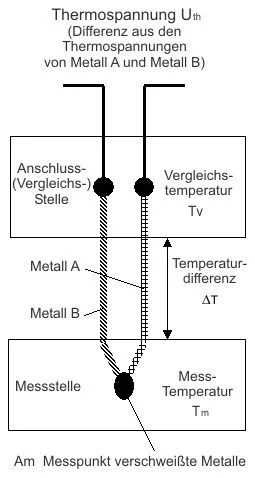
\includegraphics[width=0.5\textwidth]{bilder/thermoelement.jpg}
	\caption[Aufbau Thermoelement]{Aufbau eines Thermoelements}
	\label{fig:thermoelement}
\end{figure}


	      \end{itemize}
\end{description}